\subsection{Adding In Between Chains}

In the lower right qudrant: Period adding in between chains.

Along the chains: No ``Type B'' parameter regions, only ``Type A''.
They can overlap.
Cycle at point $A_{19}$: $\Cycle{\L^{10}\B^9}$, at point $C_{19}$: $\Cycle{\L^9\R^{10}}$.
The parameter regions overlap and both cycles coexist at point $B_{19}$.
Hard to visualize, because they have the same period.

\begin{figure}
    \centering
    \begin{subfigure}{0.4\textwidth}
        \centering
        \includegraphics[width=\textwidth]{70_030_SearchAdding_quad2/2D_Period_LowerRight/result.png}
        \caption{Full}
        %        \label{fig:final.period.whole.full}
    \end{subfigure}
    \begin{subfigure}{0.4\textwidth}
        \centering
        \includegraphics[width=\textwidth]{70_030_SearchAdding_quad2/2D_Period_LowerRight_Zoomed/result.png}
        \caption{Zoomed-In}
        %        \label{fig:final.period.whole.halved}
    \end{subfigure}
    \caption{2D Scans of Periods of Lower Right Quarter Of Quad2 Model}
\end{figure}

\begin{figure}
    \centering
    \includegraphics[width=0.6 \textwidth]{70_030_SearchAdding_quad2/2D_Regions_LowerRight_Zoomed/result.png}
    %        \label{fig:final.period.whole.halved}
    \caption{2D Scans of Period Regions in Lower Right Of Quad2 Model}
\end{figure}

\begin{figure}
    \centering
    \begin{subfigure}{0.4\textwidth}
        \centering
        \includegraphics[width=\textwidth]{70_030_SearchAdding_quad2/1D_Period_LowerRight_B18_C19/result.png}
        \caption{Between $B_{18}$ and $C_{19}$}
        %        \label{fig:final.period.whole.full}
    \end{subfigure}
    \begin{subfigure}{0.4\textwidth}
        \centering
        \includegraphics[width=\textwidth]{70_030_SearchAdding_quad2/1D_Period_LowerRight_C20_C19/result.png}
        \caption{Between $C_{20}$ and $C_{19}$}
        %        \label{fig:final.period.whole.halved}
    \end{subfigure}
    \caption{1D Scans of Periods of Lower Right Quarter Of Quad2 Model}
\end{figure}

\begin{figure}
    \centering
    \begin{subfigure}{0.3\textwidth}
        \centering
        \includegraphics[width=\textwidth]{70_030_SearchAdding_quad2/Cobweb_LowerRight_A19/result.png}
        \caption{At $A_{19}$}
        %        \label{fig:final.period.whole.full}
    \end{subfigure}
    \begin{subfigure}{0.3\textwidth}
        \centering
        \includegraphics[width=\textwidth]{70_030_SearchAdding_quad2/Cobweb_LowerRight_B19/result.png}
        \caption{At $B_{19}$}
        %        \label{fig:final.period.whole.full}
    \end{subfigure}
    \begin{subfigure}{0.3\textwidth}
        \centering
        \includegraphics[width=\textwidth]{70_030_SearchAdding_quad2/Cobweb_LowerRight_C20/result.png}
        \caption{At $C_{19}$}
        %        \label{fig:final.period.whole.halved}
    \end{subfigure}
    \caption{Cobwebs at Selected Points of Upper Left Quarter Of Quad2 Model}
\end{figure}
